%\documentclass[spanish]{beamer}

\documentclass{beamer}
\usepackage{pgf,pgfpages}
%\pgfpagesuselayout{4 on 1}[letterpaper,landscape,border shrink=0.5in]
\usepackage{algorithm,algorithmic}
%\usepackage{algorithm,algorithmicx}
%\usepackage[noend]{algpseudocode}
\usepackage{listings}
\lstset{basicstyle=\ttfamily,
	showstringspaces=false,
	commentstyle=\color{red},
	literate={á}{{\'a}}1
	{ã}{{\~a}}1
	{é}{{\'e}}1
	{ó}{{\'o}}1
	{í}{{\'i}}1
	{ñ}{{\~n}}1
	{¡}{{!`}}1
	{¿}{{?`}}1
	{ú}{{\'u}}1
	{Í}{{\'I}}1
	{Ó}{{\'O}}1
}

\usepackage{beamerthemesplit}
\usepackage{color}
\usepackage[utf8]{inputenc}
\usepackage[spanish]{babel}
%\usepackage[latin1]{inputenc}
%\usepackage[pdftex]{graphicx}
%\usepackage{algorithm}
%\usepackage{algorithmic-C}
%\usepackage{algorithmic}
\usepackage{amsthm}
\usepackage{multicol}
\usepackage{multirow}
\usepackage{fancyvrb,relsize}
\usepackage{hhline}
\usepackage{tikz}
\usetikzlibrary{trees, shapes, calc}
\newcommand{\inputTikZ}[2]{%
	\scalebox{#1}{\input{#2}}
}

\usetheme{Warsaw} %Gueno
%\usetheme{Darmstadt} %OK!
% \usetheme{Frankfurt} %OK!
%\usetheme{Goettingen}
%\usetheme{Dresden}
%\usetheme{JuanLesPins} %OK!!
%\usetheme{Marburg}
%\usetheme{Montpellier}
%\usetheme{Rochester} %sobrio
%\usetheme{Singapore}
%\usetheme{Szeged}

%\usecolortheme{albatross}
%\usecolortheme{seahorse}
%\usecolortheme{beetle}
%\usecolortheme{crane}
%\usecolortheme{dolphin}
%\usecolortheme{dove}
%\usecolortheme{fly}
%\usecolortheme{lily} %Gueno
\usecolortheme{orchid}%Gueno
%\usecolortheme{rose}
%\usecolortheme{seagull}
%\usecolortheme{whale}


\DefineVerbatimEnvironment%
      {VerbatimNN}%
      {Verbatim}%
      {fontsize=\relsize{-1}}
\DefineVerbatimEnvironment%
      {VerbatimNNN}%
      {Verbatim}%
      {fontsize=\relsize{-2}}

\DefineVerbatimEnvironment%
      {VerbatimPseudo}%
      {Verbatim}%
      {numbers=left, fontsize=\relsize{-1}}
\DefineVerbatimEnvironment%
      {VerbatimPseudoReduced}%
      {Verbatim}%
      {numbers=left, fontsize=\relsize{-2}}
\DefineVerbatimEnvironment%
      {VerbatimPseudoReduced2}%
      {Verbatim}%
      {numbers=left, fontsize=\relsize{-3}}
\DefineVerbatimEnvironment%
      {VerbatimC}%
      {Verbatim}%
      {commandchars=@ªº, numbers=left, fontsize=\relsize{-1}}
\DefineVerbatimEnvironment%
      {VerbatimReducedC}%
      {Verbatim}%
      {commandchars=@ªº, numbers=left, fontsize=\relsize{-2}}
\DefineVerbatimEnvironment%
      {VerbatimReduced2C}%
      {Verbatim}%
      {commandchars=@ªº, numbers=left, fontsize=\relsize{-3}}



%\AtBeginSubsection[]
%{
% \begin{frame}
% \frametitle{Sinopsis}
% Aqui decides: cada seccion y subseccion:
% \tableofcontents[currentsection,currentsubsection]
 %O solamente la seccion (Solo uno de ellos)
%\tableofcontents[currentsection]
% \end{frame}
%}

% Si quieres que todo por default aparezca de poco en poco
% descomenta esta linea
%\beamerdefaultoverlayspecification{<+->}

\setbeamertemplate{footline}{\hfill\insertframenumber/\inserttotalframenumber}
\setbeamertemplate{navigation symbols}{}

\setbeamercovered{transparent}

\title{ELO320 - Estructuras de Datos y Algoritmos\\Introducción a C\\Arreglos en C}
%\subtitle{Ingeniería Civil Telemática UTFSM}
\author{Dr. Nicolás Gálvez R.\\{\small nicolas.galvez@usm.cl}}
\institute{Ing. Civil Telemática - Departamento de Electrónica}
\titlegraphic{
\includegraphics[scale=.13]{images/logoutfsm}}
\date{1er Semestre 2025}

\begin{document}

\frame{\titlepage}

%\section*{Sinopsis}
%\frame{  \frametitle{Sinopsis}\tableofcontents[pausesections]}
%
% Pedir 10 datos
% funcion promedio
% funcion desviación estandar
% funcion mayor
% funcion menor
% funcion ordenar de menor a mayor
% arreglo bidimensional
% desafío: string
% pedir nombre
% contar cada letra. 


\part{Clase Activa}
\section{Clase Activa}
\begin{frame}[fragile]{Clase Activa: Módulo 1}
\begin{exampleblock}{Ejercicio 1.1}
Cree una función que reciba como parámetro un arreglo de enteros y el tamaño de éste, y luego solicite al usuario esa cantidad de valores, necesarios, para rellenar este arreglo. Puede usar una de las dos siguientes declaraciones:
\begin{lstlisting}[language=C, basicstyle=\scriptsize]
void add_datos(int arreglo[], int tam);

void add_datos(int * arreglo, int tam);
\end{lstlisting}
\end{exampleblock}

{\tiny Aprendemos: Definir un arreglo, recorrer un arreglo, rellenar un arreglo. Paso por referencia.}
\end{frame}

\begin{frame}[fragile]{Clase Activa: Módulo 1}
\begin{exampleblock}{Ejercicio 1.2}
Cree una función que reciba como parámetro un arreglo de enteros y el tamaño de éste, y luego muestre por pantalla los valores almacenados en dicho arreglo. Puede usar una de las dos siguientes declaraciones:
\begin{lstlisting}[language=C, basicstyle=\scriptsize]
void imprimir_datos(int arreglo[], int tam);

void imprimir_datos(int * arreglo, int tam);
\end{lstlisting}
\end{exampleblock}

{\tiny Aprendemos: Definir un arreglo, recorrer un arreglo, rellenar un arreglo. Paso por referencia.}
\end{frame}

\begin{frame}[fragile]{Clase Activa: Módulo 1}
\begin{exampleblock}{Ejercicio 1.3}
Cree programa que declare un arreglo de enteros de un tamaño solicitado al usuario por pantalla. Luego, debe, en conjunto con el usuario, rellenar el arreglo y mostrar por pantalla su contenido. \textbf{Utilice las funciones creadas en los ejercicios 1.1 y 1.2}.
\end{exampleblock}
 
{\tiny Aprendemos: Definir un arreglo, recorrer un arreglo, rellenar un arreglo. Paso por referencia.}
\end{frame}

\begin{frame}[fragile]{Clase Activa: Módulo 2}
\begin{exampleblock}{Ejercicio 2.1}
Cree y utilice una función que reciba como parámetro un arreglo de enteros y el tamaño de éste, y luego calcule el promedio entre todos los valores almacenados en dicho arreglo. Puede usar una de las dos siguientes declaraciones:
\begin{lstlisting}[language=C, basicstyle=\scriptsize]
float promedio(int arreglo[], int tam);

float promedio(int * arreglo, int tam);
\end{lstlisting}
\end{exampleblock}

{\tiny Aprendemos: Operar sobre un arreglo, recorrer un arreglo.}
\end{frame}


\begin{frame}[fragile]{Clase Activa: Módulo 2}
\begin{exampleblock}{Ejercicio 2.2}
Cree y utilice una función que reciba como parámetro un arreglo de enteros y el tamaño de éste, y luego calcule la desviación estándar entre todos los valores almacenados en dicho arreglo. Puede usar una de las dos siguientes declaraciones:
\begin{lstlisting}[language=C, basicstyle=\scriptsize]
float desviacion(int arreglo[], int tam);

float desviacion(int * arreglo, int tam);
\end{lstlisting}

$$ \sigma = \sqrt{\frac{\sum_{i=1}^{n}(x_i - \bar{x})^2}{n-1}}$$
\end{exampleblock}

{\tiny Aprendemos: Operar sobre un arreglo, recorrer un arreglo.}
\end{frame}

\begin{frame}[fragile]{Clase Activa: Módulo 2}
\begin{exampleblock}{Ejercicio 2.3}
Cree y utilice una función que reciba como parámetro un arreglo de enteros y el tamaño de éste, y luego calcule la varianza entre todos los valores almacenados en dicho arreglo. Puede usar una de las dos siguientes declaraciones:
\begin{lstlisting}[language=C, basicstyle=\scriptsize]
float varianza(int arreglo[], int tam);

float varianza(int * arreglo, int tam);
\end{lstlisting}

$$ V = \sigma^2 $$
\end{exampleblock}

{\tiny Aprendemos: Operar sobre un arreglo, recorrer un arreglo.}
\end{frame}

\begin{frame}[fragile]{Clase Activa: Módulo 2}
\begin{exampleblock}{Ejercicio 2.4}
Cree y utilice una función que reciba como parámetro un arreglo de enteros y el tamaño de éste, y luego entregue el arreglo ordenado de menor a mayor en el arreglo original. Puede usar una de las dos siguientes declaraciones:
\begin{lstlisting}[language=C, basicstyle=\scriptsize]
void sort(int arreglo[], int tam);

void sort(int * arreglo, int tam);
\end{lstlisting}
\end{exampleblock}

{\tiny Aprendemos: Operar sobre un arreglo, recorrer un arreglo.}
\end{frame}

\begin{frame}[fragile]{Clase Activa: Módulo 2}
\begin{exampleblock}{Ejercicio 2.5}
Cree y utilice una función que reciba como parámetro un arreglo de enteros y el tamaño de éste, y luego entregue el menor valor del arreglo. Puede usar una de las dos siguientes declaraciones:
\begin{lstlisting}[language=C, basicstyle=\scriptsize]
int menor(int arreglo[], int tam);

int menor(int * arreglo, int tam);
\end{lstlisting}
\end{exampleblock}

{\tiny Aprendemos: Operar sobre un arreglo, recorrer un arreglo.}
\end{frame}

\begin{frame}[fragile]{Clase Activa: Módulo 2}
\begin{exampleblock}{Ejercicio 2.6}
Cree y utilice una función que reciba como parámetro un arreglo de enteros y el tamaño de éste, y luego entregue el mayor valor del arreglo. Puede usar una de las dos siguientes declaraciones:
\begin{lstlisting}[language=C, basicstyle=\scriptsize]
int mayor(int arreglo[], int tam);

int mayor(int * arreglo, int tam);
\end{lstlisting}
\end{exampleblock}

{\tiny Aprendemos: Operar sobre un arreglo, recorrer un arreglo.}
\end{frame}


\begin{frame}[fragile]{Clase Activa: Módulo 3}
\begin{exampleblock}{Ejercicio 3.1}
Cree un programa que solicite un tamaño $m$ y $n$, y luego defina un arreglo bidimensional de enteros con dichos valores.

\end{exampleblock}

{\tiny Aprendemos: Arreglo bidimensional.}
\end{frame}

\begin{frame}[fragile]{Clase Activa: Módulo 3}
\begin{exampleblock}{Ejercicio 3.2}
Cree una función que reciba como parámetros un arreglo bidimensional, y sus dimensiones $m$ y $n$. La función debe permitir rellenar dicho arreglo. Puede usar una de las dos siguientes declaraciones:
\begin{lstlisting}[language=C, basicstyle=\scriptsize]
void add_datos_2(int arreglo[][n], int m, int n);

void add_datos_2(int ** arreglo, int m, int n);
\end{lstlisting}
\end{exampleblock}

{\tiny Aprendemos: Arreglo bidimensional. Recorrido bidimensional.}
\end{frame}


\begin{frame}[fragile]{Clase Activa: Módulo 3}
\begin{exampleblock}{Ejercicio 3.3}
Cree una función que reciba como parámetros dos arreglos bidimensionales de igual dimensión, y el valor de sus dimensiones $m$ y $n$. Considerando que ambos arreglos pueden ser visto como matrices, la función debe calcular la suma de ambas de matrices y almacenar dicho resultado en alguna de las dos matrices pasadas como parámetros. Puede usar una de las dos siguientes declaraciones:
\begin{lstlisting}[language=C, basicstyle=\scriptsize]
void suma(int m1[][], int m2[][n], int m, int n);

void suma(int ** m1, int ** m2, int m, int n);
\end{lstlisting}
\end{exampleblock}

{\tiny Aprendemos: Arreglo bidimensional. Recorrido bidimensional.}
\end{frame}


\begin{frame}[fragile]{Clase Activa: Módulo Desafío}
\begin{exampleblock}{Ejercicio Desafío}
Cree un programa que solicite al usuario ingresar una palabra. El programa debe determinar si la palabra es palíndroma o no. Utilice funciones para hacer su trabajo más ordenado y sencillo. Recuerde que una palabra es palíndroma si se lee de igual forma de izquierda a derecha como de derecha a izquierda.
\bigskip

\texttt{reconocer} es palíndroma. \texttt{programar} no es palíndroma.

\end{exampleblock}
{\tiny Aprendemos: Strings, Arreglo de Caracteres. Recorrido Inverso.}
\end{frame}


\begin{frame}
\centering \Huge Información de Vital Importancia para la Clase Activa\footnote{Depende exclusivamente de uds. leerla y comprenderla.}.
\end{frame}
%\section{Funciones}
%\begin{frame}[fragile]{Funciones en C}
%\begin{itemize}
%	\item Encapsula código.
%	\item Permite reutilizar código.
%	\item Se pueden compilar por separado.
%	\item Retorna siempre un tipo de dato específico. 
%\end{itemize}
%\end{frame}
%
%\begin{frame}[fragile]{Funciones en C}
%\begin{itemize}
%	\item Se puede separar interfaz (prototipo) de implementación.
%	\item \textbf{Interfaz (prototipo):} Sólo define existencia y formato de función. Suficiente para ser invocada.
%	\begin{exampleblock}{C}
%	\begin{lstlisting}[language=C, basicstyle=\tiny]
%//tipo_retorno funcion(parametros con o sin nombre);
%float potencia(float a, float b);
%//....
%
%calculo = x * potencia(y, 2.5);
%\end{lstlisting}\end{exampleblock}
%\end{itemize}
%\end{frame}
%
%\begin{frame}[fragile]{Funciones en C}
%\begin{itemize}	
%	\item \textbf{Implementación:} Define implementación de código de función.
%	\begin{exampleblock}{C}
%\begin{lstlisting}[language=C, basicstyle=\tiny]
%/*tipo_retorno funcion(parametros con nombre) {
%*	Implementacion...
%}*/
%
%float potencia(float a, float b) {
%	return power(a,b);
%}
%\end{lstlisting}\end{exampleblock}
%\end{itemize}
%\end{frame}
%
%\begin{frame}[fragile]{Funciones en C}
%\begin{itemize}
%	\item Si se utiliza solamente la implementación, está tiene que estar definida \textbf{antes} de la función que la utiliza.
%	\item Si se utiliza el prototipo, es éste el que debe estar defindo \textbf{antes} de la función que la usa.
%	\item Prototipo + Implementación: libertad de ubicación de la implementación $\rightarrow$ diferentes archivos.
%\end{itemize}
%\end{frame}
%
%\begin{frame}[fragile]{Funciones en Python}
%\begin{itemize}
%	\item \textbf{Python} sólo permite implementación, sin prototipos.
%\begin{block}{Python}
%	\begin{lstlisting}[language=Python, basicstyle=\scriptsize]
%def nombre_funcion(parametros):
%    #...Implementacion
%    return <expresion>
%	\end{lstlisting}
%\end{block}
%	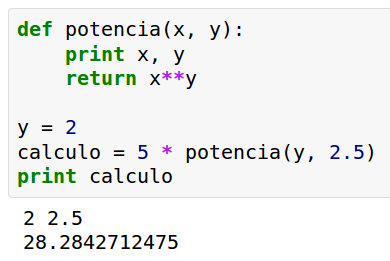
\includegraphics[width=.65\linewidth]{images/funcion-python.png}
%\end{itemize}
%\end{frame}
%
%
%
%\subsection{Macros y Constantes}
%
%\begin{frame}[fragile]{Macro}
%Una macro es un valor o conjuntos de instrucciones constantes que se definen a nivel de preprocesamiento. No es una variable y no puede ser modificada. 
%
%\begin{exampleblock}{C}
%\begin{lstlisting}[language=C, basicstyle=\scriptsize, escapeinside={|}{|}]
%#include<stdio.h>
%#define MACRO 10
%
%int main(){
%	int a = 5;
%	printf("|\%|"s\n", a*MACRO);
%}
%\end{lstlisting}\end{exampleblock}
%\end{frame}
%
%\begin{frame}[fragile]{Constante}
%Una variable constante es aquella que se declara con el keyword \textbf{const}, e implica que ésta no puede ser modificada. Tiene todo el resto de las propiedades de una variable común.
%
%\begin{exampleblock}{C}
%\begin{lstlisting}[language=C, basicstyle=\scriptsize, escapeinside={|}{|}]
%#include<stdio.h>
%
%int main(){
%	const int a = 5;
%	a = 10; //¿Cómo actúa el compilador?
%	printf("|\%|d\n", a);
%}
%\end{lstlisting}\end{exampleblock}
%\end{frame}
%
%\subsection{Ámbito}
%
%
%\begin{frame}[fragile]{Ámbito (Scope)}
%Las funciones (includa main) definen el alcance de las variables, llamado \textbf{ámbito}, vale decir, el segmento en el cual existen y pueden ser usadas $\rightarrow$ entre \{ y \}.
%
%\begin{exampleblock}{C}
%\begin{lstlisting}[language=C, basicstyle=\scriptsize, escapeinside={|}{|}]
%#include<stdio.h>
%
%void saludo(){ // var i sirve sólo dentro de función saludo.
%	int i = 5;
%	printf("Hola alumno numero |\%|d", i);
%}
%
%int main(){// var a sirve sólo dentro de función main. 
%	int a = 10;
%	saludo();
%	printf("|\%|d\n", a);
%	return 0;
%}
%\end{lstlisting}\end{exampleblock}
%\end{frame}
%
%\subsection{Var. Global y Var. Local}
%
%\begin{frame}[fragile]{Variable local}
%Una variable local, es aquella que está definida dentro de un ámbito determinado, vale decir, entre llaves \{ y \}.\\
%\bigskip
%
%Esto aplica para todo elemento que contenga llaves, incluida funciones y estructuras de control. 
%\end{frame}
%
%\begin{frame}[fragile]{Variable local}
%\begin{exampleblock}{C}
%\begin{lstlisting}[language=C, basicstyle=\scriptsize, escapeinside={|}{|}]
%#include<stdio.h>
%
%int main(){// var a sirve sólo dentro de función main. 
%	int a = 10;
%
%	if(a==10){
%		int b = 1;
%		printf("|\%|d |\%|d\n", a, b);
%	}
%	// ¿Qué pasa con la variable b?
%	printf("|\%|d |\%|d\n", a, b); 
%
%	return 0;
%}
%\end{lstlisting}\end{exampleblock}
%\end{frame}
%
%
%\begin{frame}[fragile]{Variable Global}
%Una variable global, es aquella que está definida \textbf{fuera de cualquier} ámbito.\\
%\bigskip 
%
%Puede ser llamada, modificada y utilizada desde cualquier ámbito, siempre y cuando \textbf{no exista una variable local} con el mismo nombre. 
%
%\end{frame}
%
%\begin{frame}[fragile]{Variable Global}
%
%\begin{exampleblock}{C}
%\begin{lstlisting}[language=C, basicstyle=\scriptsize, escapeinside={|}{|}]
%#include<stdio.h>
%
%int a=1; //global
%int b=2; //global
%
%int main(){
%	int a = 10; //local
%	b++;
%	printf("|\%|d |\%|d\n", a, b);//¿Qué imprime? 
%	return 0;
%}
%\end{lstlisting}\end{exampleblock}
%
%En python, no se pueden modificar variables globales dentro de una función.
%\end{frame}

\section{Arreglos}
\subsection{Arreglos}
\begin{frame}[fragile]{Arreglos}
\begin{itemize}
\item \textbf{Arreglo:} Conjunto homogéneo y ordenado de un tipo de datos.
\item Se identifican por su posición relativa mediante un \emph{índice} encerrado con paréntesis cuadrado ([], parte de índice 0).
\begin{lstlisting}[language=C,basicstyle=\scriptsize,escapeinside={|}{|}]
int arr[6]; //6 enteros creados en arr.
arr[3] = 222; //Al cuarto elemento de arr se le asigna un 222.
\end{lstlisting}
\begin{center}

\includegraphics[width=.75\linewidth]{images/array.png}
\end{center}
\end{itemize}
\end{frame}

\subsection{Strings}
\begin{frame}[fragile]{Arreglos}
\begin{itemize}
\item \textbf{String:} Estructura de datos para representar palabras.
\item Arreglo de \texttt{char} y el caracter \texttt{'\textbackslash 0'}.
\begin{lstlisting}[language=C,basicstyle=\scriptsize,escapeinside={|}{|}]
// Los string terminan con '\0' (fin de string) 
// '\0' ocupa 1 char en el string.
char str[6] = "hola"; //String de largo máximo 5. 
str[3] = 'i'; // ¿Qué hace? 
printf("|\%|s\n", str);
\end{lstlisting}
\begin{center}

\includegraphics[width=.75\linewidth]{images/string.png}
\end{center}


\item Veremos más sobre strings las próximas clases. 	
\end{itemize}
\end{frame}

\subsection{Arreglos Multidimensionales}
\begin{frame}[fragile]{Arreglos Multidimensionales e Inicialización}
Además, se pueden definir arreglos multidimensionales.\\
\bigskip

También, los arreglos pueden ser inicializados utilizando \{ y \}.
\begin{exampleblock}{C}
\begin{lstlisting}[language=C,basicstyle=\scriptsize,escapeinside={|}{|}]
#include<stdio.h>

int main(){
	char nom[10] = "Camilo";
	char a[5][20] = {"Juan", "Francisco", "Pedro"};	
	int b[3][3] = {{1,2,3}, {4,5,6}, {7,8,9}}, i, j;

	for(i=0;i<3;i++){
		for(j=0;j<3;j++) //¿Qué pasó con las llaves? 
			printf("|\%|d ", b[i][j]);
		printf("\n");
	}
}
\end{lstlisting}
\end{exampleblock}
\end{frame}

\begin{frame}[fragile]{Recorrer un arreglo}
Podemos utilizar cualquiera de las estructuras de control iterativas para recorrerlos. 
\begin{exampleblock}{C}
\begin{lstlisting}[language=C,basicstyle=\scriptsize,escapeinside={|}{|}]
#inclede<stdio.h>

int main(){
	int i;
	float a[5];
	
	for(i=0;i<5;i++){
		float val; //¿Cuántas veces nace y muere val?
		scanf("|\%|f", &val);
		a[i]=val;
	} //¿Cómo reducir este código?

}
\end{lstlisting}
\end{exampleblock}
\end{frame}

%\begin{frame}[fragile]{Recorrer un arreglo}
%Practiquen con los siguientes ejercicios:
%\begin{itemize}
%\item Calcular el factorial de un número dado.
%\item Ordenar de mayor a menor un arreglo de una dimensión.
%\item Encontrar el mayor elemento en un arreglo de dos dimensiones.
%\item Calcular el promedio de los elementos en un arreglo bidimensional.
%\item Imprimir en orden inverso los elementos de un arreglo. 
%\item Imprimir todas las letras mayúsculas y minúsculas del alfabeto (ver Código ASCII).
%\end{itemize}

%\end{frame}


%\begin{frame}[fragile]{Tipos de Datos Abstractos - Estructuras}
%\begin{itemize}
%	\item Conjunto (posiblemente) heterogéneo de elementos de datos (e.g.: estructuras y clases).
%	\item Cada elemento individual (campo, miembro o atributo) identificado con un nombre. 
%	\item Encapsulamiento de información.
%	\item Ejemplo:
%	\begin{lstlisting}[language=C++]
%struct empleado {
%    char nombre[40];
%    char ap_paterno[40];
%    char ap_materno[40];
%    float sueldo;
%};
%//...
%empleado e1, e2;
%
%//Acceso a atributos con operador '.'
%e1.sueldo = 550000.00;
%strcpy(e1.nombre, "Juan");
%	\end{lstlisting}
%\end{itemize}
%\end{frame}



\end{document}
